%===================================================================================
\subsection{CU29 Mis tareas}
{
\justify
\color{blue}{\textbf{Objetivo}}
}

%------------------------------------------------------------------
\justify
Permite al Lider de proyecto y al colaborador, ver la tareas que tinen asignadas en el proyecto que estan participando.
%------------------------------------------------------------------
{
\justify
\color{blue}{\textbf{Diseño}}
}
%-------------------------------------------------------------------------------
\justify
En la figura \ref{fig:IU29} se muestra la pantalla, en donde permite al Lider de proyecto y al colaborador, ver la tareas que tinen asignadas en el proyecto que estan participando.

\begin{figure}[htb]
\centering
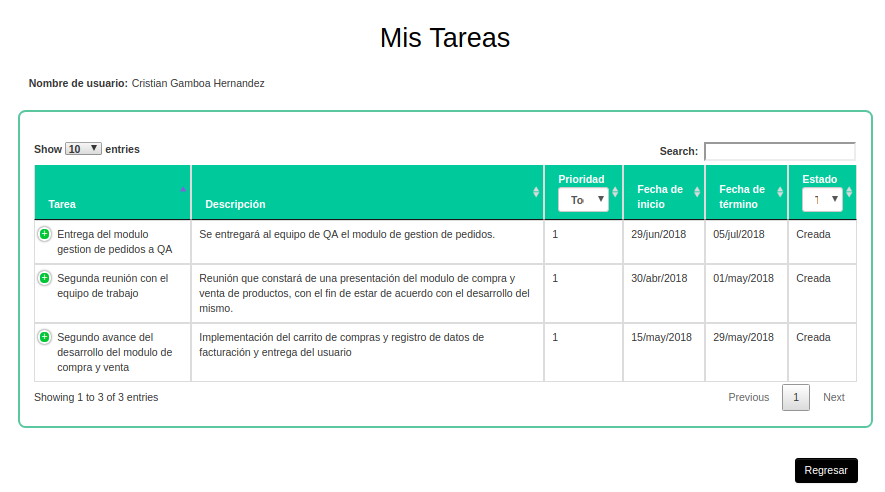
\includegraphics[width=0.8\textwidth]{./images/cu29-mis-tareas.png}
\caption{Ver estadisticas de avances de las tareas.} \label{fig:IU29}
\end{figure}

\newpage